% !TEX root = ../CedricDe Schepper2023_Thesis.tex

\section{Results / Evaluation}\label{sec:results}

In order to evaluate the results from the experiment, we have to verify whether the phases perform their objective as described. Firstly, does the initialisation phase succeed in generating a `feasible´ solution namely one without or with a minimal number of hard constraint violations? Secondly, does the optimisation phase succeed in transforming the initial solution into one with an acceptable solution?

All experiments reported in the following subsections were conducted on a personal computer running on a Intel Core i7-6700HQ processer with 16GB of RAM memory.

\subsection{Reference solutions}

The actual exam schedules, manually created by the administration of the \acrlong{ua}, can be used as a baseline to compare the generated schedules. These exam distributions can be seen in Figures \ref{fig:manual_sem1} and \ref{fig:manual_sem2}. Most notably, the manual schedules have a focus on keeping the amount of same day exams to a minimum and having 2 or more days in between exams as much as possible. This distribution is especially visible in the schedules for \acrshort{fti}. Additionally, it can be seen that the schedule for \acrshort{fwet} contains a high amount of exam conflicts. In order to be considered a superior solution, automatically generated schedules will have to minimise the amount of exams with fewer than 2 days in between, with a focus on same day exam violations.

\begin{figure}[H]
  \centering
  \subfloat[FTI]{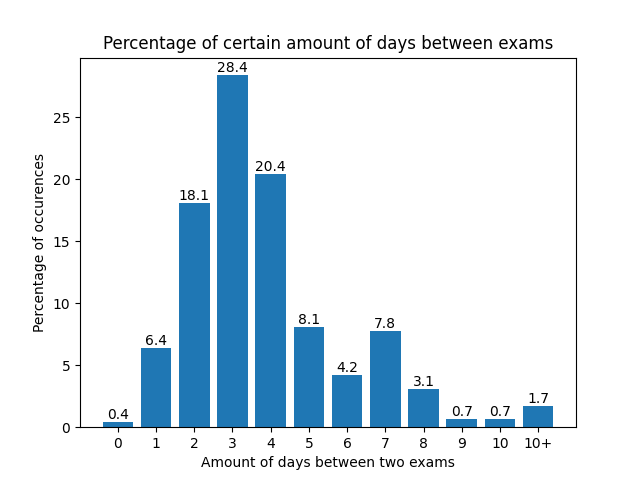
\includegraphics[width=0.5\textwidth]{images/manual/fti_sem1_percentages_manual.png}}
  \hfill
  \subfloat[FWET]{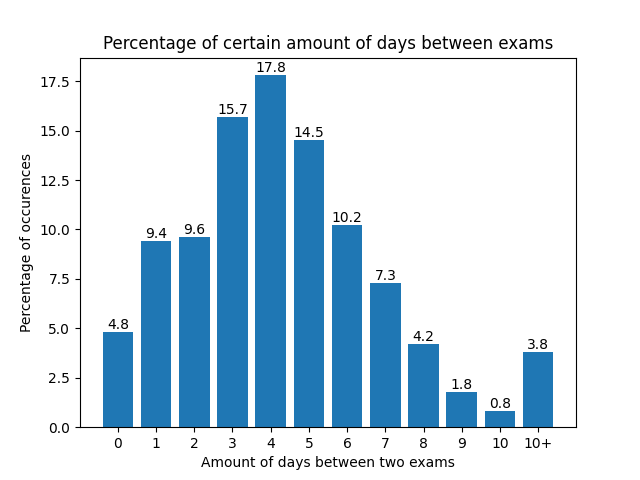
\includegraphics[width=0.5\textwidth]{images/manual/fwet_sem1_percentages_manual.png}}
  \caption{Manual exam distribution for January 2021}
  \label{fig:manual_sem1}
\end{figure}

\begin{figure}[H]
  \centering
  \subfloat[FTI]{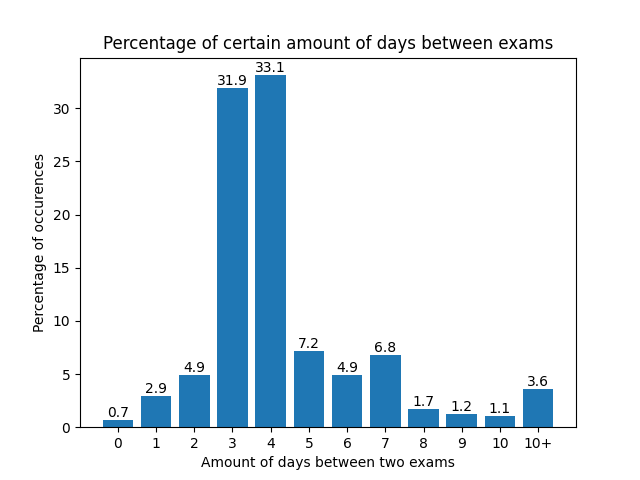
\includegraphics[width=0.5\textwidth]{images/manual/fti_sem2_percentages_manual.png}}
  \hfill
  \subfloat[FWET]{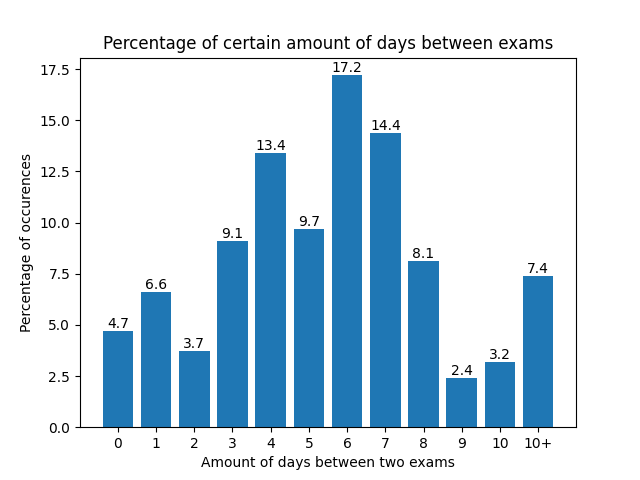
\includegraphics[width=0.5\textwidth]{images/manual/fwet_sem2_percentages_manual.png}}
  \caption{Manual exam distribution for June 2021}
  \label{fig:manual_sem2}
\end{figure}

\subsection{Initialisation phase} \label{phase_init}

In order to quantify the feasibility of a solution, it is possible to look at either the objective function or the amount of hard constraint violations. Since the objective function was adapted to contain exponents and the conflict weight having a large impact on the size of the objective, looking at the amount of hard constraint violations can provide a better perspective. By plotting the violations per iterations, the progress made by the initialisation phase can be visualised. Figure \ref{fig:violations} shows the amount of exam conflicts for students. Since all hard constraints besides the student conflicts are guaranteed, this shows the amount of hard constraints present. This that the initialisation phase is able to generate a solution for \acrshort{fti}+\acrshort{fwet} without hard constraint violations. It reaches a feasible solution after fewer than 150 iterations, generally taking under 500 seconds. 

However, Figure \ref{fig:init} shows that no attention was given to the distribution which can be confirmed by the presence of a high percentage of exams after a single day. These figures are generated by calculating the distance between each exam for every student, with the exams being sorted on exam date. For example, a student A with exams on day 1, 5, and 7 will contribute the distance between day 1 and 5, as well as the distance between day 5 and 7. This results in the student contributing to the $x = 4$ and $x = 2$ bar, respectively. We can also look at the case for a student B with conflicting exams. This can be showcased using an identical schedule compared to student A, with the addition of a conflicting exam on day 5. This results in the distances being calculated using the sequence of 1, 5, 5, and 7. Because of this, student B will contribute to $x = 4$, $x = 0$, and $x = 2$ bar, respectively.

\begin{figure}[H]
	\centering
	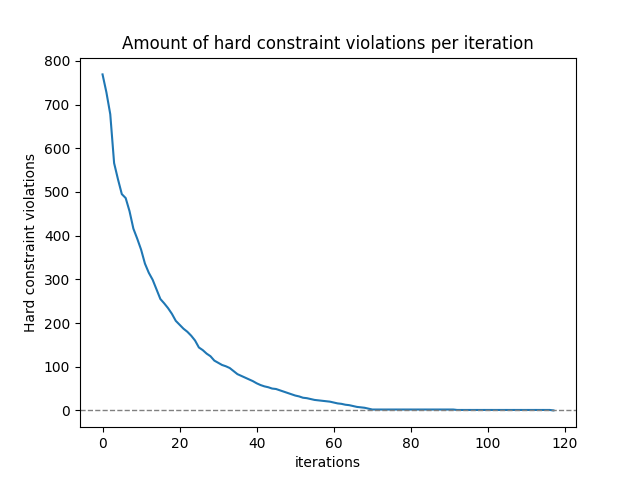
\includegraphics[width=0.5\textwidth]{images/init/conflicts.png} 
	\caption{Hard constraint violations}
	\label{fig:violations}
\end{figure}
% TODO add dotted line for y=0
\begin{figure}[H]
  \centering
  \subfloat[FTI]{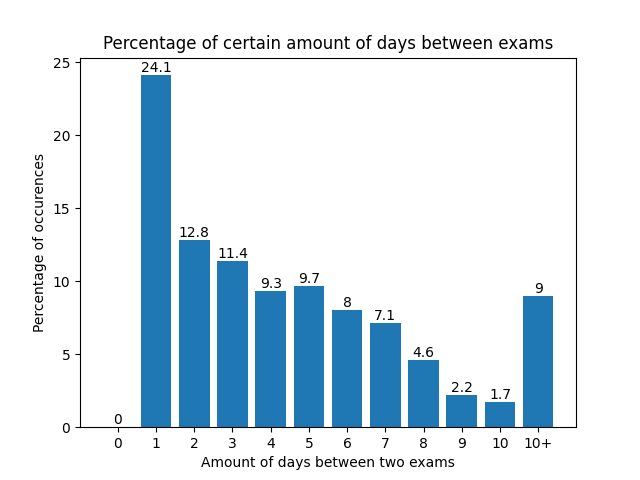
\includegraphics[width=0.5\textwidth]{images/init/fti.png}}
  \hfill
  \subfloat[FWET]{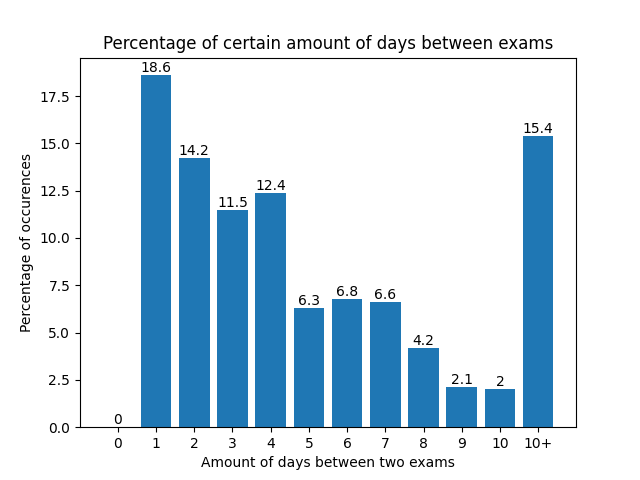
\includegraphics[width=0.5\textwidth]{images/init/fwet.png}}
  \caption{Exam distribution after initialisation phase for June 2021}
  \label{fig:init}
\end{figure}

\subsection{Optimisation phase}

While we have shown that tabu search can efficiently generate a feasible solution from the provided data set, the exam distribution will determine whether the automated schedules are superior in quality compared to the manual timetables provided by the university's administration.
% Table~\ref{tab:example} shows an example of creating a table.

% \begin{table}[h]
% 	\caption{Fictitious Results}
% 	\label{tab:example}
% 	\centering
% 	\begin{tabular}{l c c c }
% 		\hline
% 		& \textbf{Precision} & \textbf{Recall} & \textbf{F-Score} \\ \hline
% 		Technique 1 & 0.85 & 0.77 & 0.81 \\
% 		Technique 2 & 0.82 & 0.81 & 0.81 \\
% 	         Technique 3 & 0.65 & 0.93 & 0.73 \\ \hline
% 	\end{tabular}
% \end{table}

